\section{Method}
\label{method}

(TODO the history of network analysis)
%TODO computer aided network analysis <- distinction between 'verkostotutkimus' mentioned in Juuso Marttila's thesis. 
My method is computer aided social network analysis. It is one of the most implemented methods in the field of digital humanities. According to  

Quite a few textbooks have been written on (social) network analysis.\footcites[See e. g. ][or Krishna Raj P. M., Ankith Mohan and K. G. Srinivasa \textit{Practical Social Network Analysis with Python} or Xiaoming Fu et al. \textit{Social Network Analysis: Interdisciplinary Approaches and Case Studies}.]{huhtamakiEtAl}

To give some examples of the more qualitative side of method: the doctoral dissertations of both historian Marko Hakanen and historian Mirkka Lappalainen have been written using the more theoretical and qualitative methods of network analysis. Marko Hakanen studied the network of clients [lower ranking supporters] around the Count Per Brahe in the 17th century Sweden.\footcite{hakanen11} Mirkka Lappalainen on the other hand researched the Creuz family in the 17th century Sweden (and Finland).\footcite{lappalainen05}

Alongside these dissertations a master's thesis from the University of Jyväskylä Department of History and Ethnology deserves to be mentioned. In his thesis Jesse Kananen studied the of correspondence networks the rector of the Jyväskylä Seminar Karl Gabriel Leinberg. For his analysis Kananen has collected a remarkable sized dataset of 1147 letters from 487 contacts. Kananen also approaches the subject with a more qualitative stance of social network analysis.\footcite{kananen18}

Besides the subject matter, the inherent form of the graph separates our works. The dataset collected by Kananen forms an \textbf{egocentric network}, which means a kind of star shaped network with the one node on the center connected to each node on the sides. However, the links between the nodes on the sides are not taken into account (most of the time).\footcite[pp. 22-23.]{kananen18}

Despite on the quantitative sphere, the method in my thesis is still fairly simple and completely explainable. As things like machine learning and artificial intelligence (AI) are particularly popular and to a certain degree hyped at the time of writing, it is important to assess and understand the fundamentals and basics of digital and computational methods. Obviously, it is easier to understand simpler models, and therefore ask important questions. Those questions are for instance: What are the premises for this model? What kind of data is suitable for this model? What kind of interpretations can be made from the results? What is the potential problem, how to fix or adjust the model if something goes wrong or unexpectedly? On the following subsection I will go through the basis of the model.

\subsection{Defining the Network}
\label{network}
Network analysis combines mathematics, statistics and social sciences. Primarily it is based on the mathematical graph theory. A graph is a representation of the network. Graph includes \textbf{nodes} (also called vertices) and \textbf{edges} (also called links and connections).\footcites[p. 247, 248-249.]{huhtamakiEtAl}[pp. vi-vii]{RajPM2018a} If an edge exist between nodes, they are called as \textbf{neighbors}.\footcite[p. vii]{RajPM2018a}

\begin{figure}
	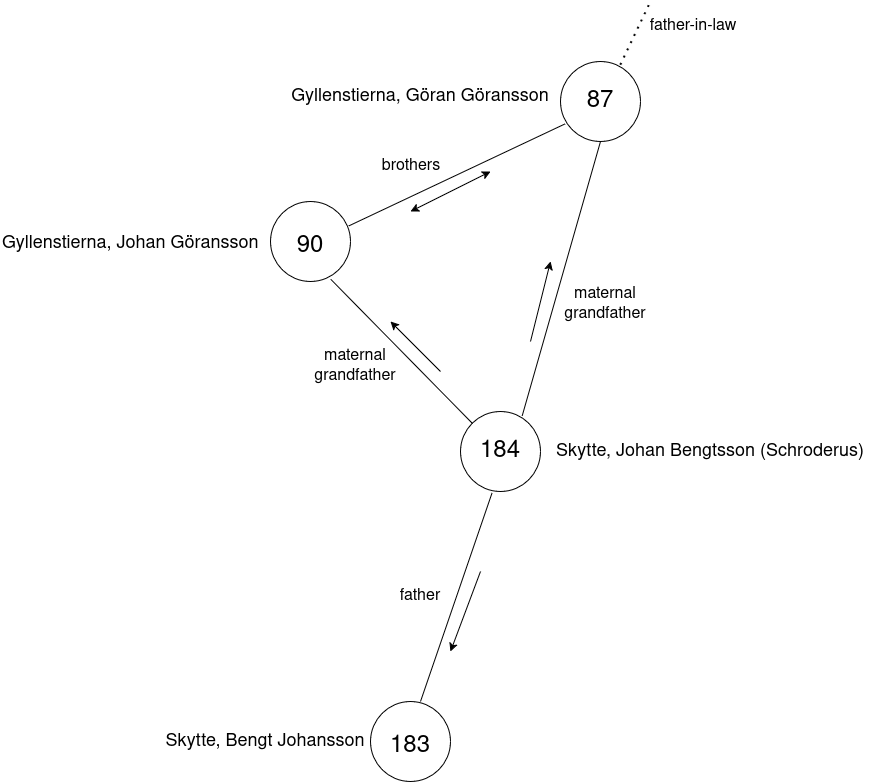
\includegraphics[scale=0.25]{example_network.drawio.png}
	\centering
	\caption[A sample from the graph]{A sample from the graph (Data by \cite{councillorsDS} graph by author)} 
	\centering
	\label{samplegraph}
\end{figure}
In this context the graph's nodes depict individual councillors with the input of name and id number. Correspondingly the edges represent the kinships between two nodes. For instance, in Figure \ref{samplegraph} we can see that Johan Bengtsson (Schroderus) Skytte (id 184) is Bengt Johansson Skytte's (id 183) father, and a maternal grandfather for Johan Göransson Gyllenstierna (id 90) and Göran Göransson Gyllenstierna (id 87). Johan and Göran Göransson are brothers, however, their father is not mentioned in the dataset. Göran Göransson also has further links in the network.

The node depicting Johan Bengtsson (Schroderus) Skytte (id 184) is a neighbor to all of the other nodes. On the contrary the node depicting Bengt Johansson Skytte (id 183) is not neighbor to Johan Göransson Gyllenstierna (id 90) or Göran Göransson Gyllenstierna (id 87). They are linked indirectly, neighbor's neighbors or formally second-order neighbors or distance two neighbors. 

A graph can be \textbf{directed} or \textbf{undirected}. In a directed graph the edges have directions, like in a correspondence network a letter has a sender and a receiver. The directions are marked with an arrow. In undirected graphs the edges are bidirectional [two way], for example a relationship between two brothers can be understood as undirected. Directed graphs have more features and a more complex structures, for instance, the degrees of inbound and outbound edges can be counted separately.\footcite[pp. 1-2.]{RajPM2018} For simplicity, the graphs presented in this work are undirected.

Calculating different statistics is a crucial part of the network analysis. One of the most important measures is the \textbf{node degree}. The node degree simply means the number of edges adjoined to a specific node.\footcite[pp. 2-3.]{RajPM2018} For example, the degree of the node depicting Johan Bengtsson (Schroderus) Skytte (id 184) is three, and the degree of the node depicting Bengt Johansson Skytte (id 183) is one. 

The \textbf{average degree} is the mean of all the node degrees of the specific graph. It is calculated by adding all the node degrees and dividing the sum with the number of nodes.\footcite[pp. 3-4.]{RajPM2018} In the case of this study, the average degree describes the average number of direct family links councillors had within the Council. The average degree of Figure \ref{samplegraph} is $\frac{1 + 3 + 2 + 3}{4} = 2.25$.

The \textbf{density} of the network is also based on the node degrees. In a dense network almost every node is connected to each other, but a sparse graph has just a few edges between the nodes. The density is calculated by dividing the number of actual edges with the maximum number of edges. The scale of density is from 0 to 1, 1 implying a \textbf{complete graph}. In the complete graph each node is adjoined to each other node.\footcite[pp. 5-6.]{RajPM2018} In practice, density is probably not the most depicting parameter of social networks because it is heavily dependant on the size of the network. 

The maximum edges–meaning the amount of all possible edges–increases rapidly with the number of nodes. Formally, the maximum edges follows the \textit{binomial coefficient}. The formula being:\footcites[p. 16.]{laininen2002}[pp. 5-6.]{RajPM2018}
\begin{equation*}
\binom{n}{k} = \frac{n!}{k!(n-k)!} = \frac{n(n-1)...(n-k+1)}{k!}
\end{equation*}
In this case $k = 2$, because two nodes share one edge. The variable n is the amount of nodes in the graph. In R environment this can be calculated easily using the function \texttt{choose(n,k)}. For example in a graph consisting of 257 nodes (the amount of the councillors in the dataset) the amount of possible edges is 32 896:
\begin{equation*}
\binom{257}{2} = \frac{257!}{2!(257-2)!}
\end{equation*}
or \texttt{choose(257,2)} with R.

In practice the rapidly growing amount of possible edges makes it inefficient to compare two graphs of different size. The number of possible edges in a graph with 100 nodes is 4 950 and in a graph with 101 nodes it is 5 050 a difference of 100 possible edges. In the context of social networks the difference is significant.

As structures graphs hold a plethora of further possibilities in representing data. For example, attributes like \textbf{weight} or \textbf{type} could be added to the graph's edges. Weight indicates the strength of the connection, in this case it could mean that a father's tie to son is stronger than the cousins tie with each other. Type indicates the nature of the relationship, such as, brother or son-in-law. The weights and types can be used in categorizing the network or counting statistics. A graph with weighted edges is called \textbf{weighted graph}.\footcite[pp. 11-12.]{RajPM2018} For simplicity the graphs presented in this work are unweighted and do not hold any attributes on the edges. 

\subsection{Implementation of the Network Analysis}
I use the combination of Python programming language and Gephi software in the data processing and analysis. Python is used for extracting the data from the councillors-dataset and formulating it in the right format: readable for Gephi. Whereas the actual network analysis: visualization and calculating statistics, is performed with Gephi. 

Python is a high level\footnote{Meaning code intended to be read and undersood by humans if compared for example with binary code written only with 0s and 1s.} programming language. Python can be used in variety of tasks including data processing, machine learning (AI models) or web development. Python is intended to be of object oriented programming style, however, it is not determined to be used only on that paradigm.\footcite[p. 1.]{pythonbook} For instance, my personal programming style is more in the imperative style. 

I selected Python due its simple syntax and ease in implementing relatively small tasks in data processing. The language is understandable and widely used amongst scientists, which makes the work replicable. To be precise the scripts are written with Python 3, exact version being Python 3.11.7.

As graphs are structures commonly used in programming, it would have been possible to conduct the actual network analysis using tools provided by Python or R\footnote{See e. g. Raj P.M., Krishna, Ankith Mohan and K.G Srinivasa \textit{Practical Social Network Analysis with Python} or Dehmer, Matthias; Shi, Frank Emmert-Streib and Yongtang Shi \textit{Computational Network Analysis with R}.}, yet, Gephi software provides a graphical user interface (GUI) and more intuitive tools for the manipulation and visualization of the graph. Furthermore, the Gephi format makes the data and graph accessible also for non programmers.

Gephi is a software for network visualization and analysis. It contains tools for manipulating, filtering, clustering and visualizing the graph. It has built in appliances for fixing errors in data and calculating necessary statistics.\footcite{gephi} Gephi reads data from text format (comma separated values .csv) or Microsoft Excel tables (XLSX), and Gephi projects are saved as .gephi files. The processed graphs and data can be exported as images or tables.  

Nonetheless, Gephi does have some weaknesses. It is not always the most intuitive to use, and especially the visual configurations of the graph causes some issues. I have encountered difficulties with the node labels (the councilor's name next to the node). Sometimes the problems lies in the Gephi settings, but if the whole software crashes when trying to make the node labels visible, the problem lies deep within the software itself. It is most likely caused because Gephi tries to connect to a non-existent graphic card. The problem must be solved while starting the program.\footnote{For Linux environments opening Gephi from command line with command "LIBGL\_ALWAYS\_SOFTWARE=1 ./gephi" can sometimes help.} 

Lastly, I use R programming language and environment for calculations and statistical analysis. R is a language and platform particularly designed for statistical analysis. It contains tools and ready-made functions for efficiently calculating and plotting statistical data.\footcite{R} The language is widely used amongst scientists. 

All of these tools are open source and free to download. In the name of replicability and transparency, all scripts written for this work available on my GitHub page.\footnote{\url{https://github.com/Heidi-Suurkaulio/mastersthesis}}

Following and modifying the steps of network analysis given by Huhtamäki and Parviainen, I listed the following six  basic steps in network analysis.\footcite[p. 258]{huhtamakiEtAl} 
The basic steps are : \begin{enumerate}
	\item Choosing the subject and data
	\item Pre processing the data for the network analysis
	\item Constructing the graph and finding possible issues and errors 
	\item Counting the statistics
	\item Deciding the layout (algorithm)
	\item Doing the interpretations
\end{enumerate}
In practice the analysis is not that straightforward, sometimes the steps 2 and 3 must be repeated and re-repeated. Yet, on some circumstances the graph is not visualized or the statistics are not deemed important. These steps will be discussed in practice below.

\subsubsection{Test Run}
To draft the structure of the graph and understand the nuances of the given data, a test run was carried out. The test run was done with a simple Python script, and no attention was paid to the temporal aspects of the network or the potential directions within the graph. The script and Gephi project used, and the visualization of the graph of the test run is available in GitHub in the TestRun folder\footnote{\url{https://github.com/Heidi-Suurkaulio/mastersthesis/tree/main/TestRun}}

The data processing was started by manually cleaning the data in LibreOffice Calc (equivalent to Microsoft Excel). The columns and rows containing information of the source material of the dataset and councillor's years active were removed. That made the structure of the data coherent and easier to manipulate with the Python script. The manually cleaned data is exported as .csv (comma separated values) file. The .csv file's header (the first line of the file) should be modified so that the column name "No." is changed to "Id" and "Family members in the council of the realm" is changed to "Family", the first one can cause an error if referenced in the Python code, the latter is inconveniently long.

The script itself reads the data from the .csv file. The connections between the councillors are separated from the "Family" column, based on the knowledge that each connection is marked with the id number of another councillor. The connections are then formatted and printed to .csv file. The connections .csv file containing values for "Source" id of the source concillor, "Target" id of target councillor, "Type" standard "Undirected", "Id" id number for the connection, "Weight" standard 1.0. Another .csv file is formatted and printed with the information of councillors' names and id numbers.

\begin{table}[h]
	\caption{Example of the connections .csv file}
	\centering
	\begin{tabular}{cccccc}
		\hline
		1 &Source, &Target, &Type, &Id, &Weight \\
		\hline
		2 &231, &228, &Undirected, &0, &1.0 \\
		\hline
		3 &231, &230, &Undirected, &1, &1.0 \\
		\hline
	\end{tabular}
\end{table}
\begin{table}[h]
	\caption{Example of the councillors .csv file}
	\centering
	\begin{tabular}{ccc}	
		\hline
		1 &Id; &Label \\
		\hline
		2 &162; &Ingemar Petri \\
		\hline
		3 &231; &Tre Rosor, Ture Jönsson \\
		\hline
	\end{tabular}
\end{table}

These .csv files are readable for Gephi. The outcome was an undirected graph of the councillors' affiliation network that had accumulated during the 160 years. The graph consisted of 261 nodes (257 real + 4 "ghosts") and 372 edges (including self loops and "ghost" nodes). The test run revealed three problems within the graph: the emergence of the empty "ghost" nodes, \textbf{parallel edges} and thirdly \textbf{self loops}. 

The "ghost" nodes were excess nodes with no name and only an id number and one or two connections in the graph. They were due to the references to the data points removed from the original dataset, and therefore can be ignored. The ghosts are discussed further in the subsection \ref{sources}. However, the more essential problem were parallel edges and self loops.

If multiple edges share the same source and destination nodes, they are called parallel edges.\footcite[pp. 14-15.]{RajPM2018} These occur because one relationship, such as father and son, is sometimes marked parallel in the dataset. For example, in the case of Göran Göransson Gyllenstierna (id 87) the relatives are "Maternal Grandfather 184, Brother 90, Father-in-law 3, ...", and the same relationship is found in his grandfather's Johan Bengtsson (Schroderus) Skytte's (id 184) links: "Son 183, Grandson through daughter 87". Yet, the connection to Göran Göransson's brother Johan Göransson Gyllenstierna (id 90) is not marked in the grandfathers links. This means that the node of Göran Göransson Gyllenstierna (id 87) has one excess link compared to his brother's node. The case is visualized in the Figure 2.

\begin{figure}[h]
	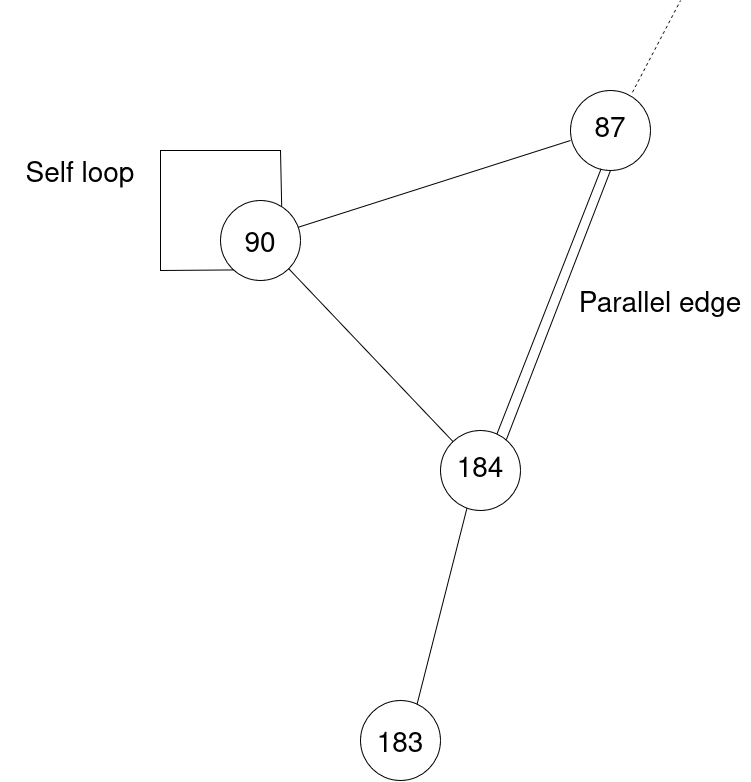
\includegraphics[scale=0.20]{double_link.drawio.png}
	\centering
	\caption{Visualization of the parallel edge and self loop} 
	\centering
\end{figure}

These duplicate edges would cause bias to the calculation of the node degrees and any statistics based on them. A node degree is a sum of all the edges connected to one node, and if the relationships are inconsistently marked with one or two edges, the factually similar nodes would get different degrees. These inconsistent node degrees would accumulate when counting the average degrees an so forth. The problem of parallel edges is widely recognized in the field of network analysis, and therefore Gephi does have some builtin features for handling it.

While importing data to Gephi (on Import Spreadsheet) the strategy for merging the parallel edges can be chosen. One option is, for example, placing the sum or average of the parallel edges in the edge's degree, yet using only one connection to to represent the edge in the graph. In this context a more simple solution was chosen, with the option "First" Gephi will use only the first connection between two nodes ignoring any latter ones. This will reduce the amount of connections from 698 found in the connections.csv to only 372.

Self loops occur when one node has–for some reason or another–a connection to itself.\footcite[p. 13.]{RajPM2018} Similarly to the parallel edges, they cause bias to the node degrees. In this graph a self loop can be found at least on the node with id 5 and id 90. In the case of id 5: Gustaf Axelsson Baner, his relatives are "Father 4, Father-in-law 217, Brother 9, Sons 5, 7, 8, 10, Sons-in-law 152 and 197", and similarly with id 90: Johan Göransson Gyllenstierna his family reads "Maternal Grandfather 184, Brother 90". These self loops are most likely caused by a typo in the dataset, because it is reasonable to assume that none is a son or brother to themselves.
 
Gephi does have a switch whether or not self loops are allowed in the graph, and it can automatically remove them based on the preference. The self loops are present in the test run graph alongside with the ghost nodes, yet those will be removed from the subsequent analysis. To highlight the ghosts they are colored cray, and the four nodes referred as an example here are colored red in the test run graph.

The last step in the preparation of the network analysis is the selection of the layout algorithm. For the test run an algorithm called Yifan Hu was used with default configurations except parameter theta set to 2.0. Then layout option "noOverlap" was chosen to separate possibly overlapping nodes, and some further manual placement of the nodes was done to make the graph more readable. The outcome was visually somewhat dense network in the middle and mostly unconnected isolated nodes around it. 

\subsection{Fitting Modern Model on a Historical Time Period}
\label{background}
\begin{quote}
	Every model is an approximation.\\
	All models are wrong; some models are useful.\\
	(\cite[prefix]{statisticsfor})
\end{quote}

George Box with his colleagues have collected aphorisms depicting statistics and model building to the prefix of their book. Those aphorisms emphasize the ambiguous nature of (statistical) models. A graph is elementally a generalizing and simplifying model of complex social networks within the Swedish Council of the Realm. Yet, when bulding any kinds of (computational) models, decisions between the complexity and abstraction must be made. In fact besides too simplifying models, too complex or overfitted ones are a problem on their own.\footnote{TODO} Due that, one of the most important question is what factors to include and and what to exclude. Yet, a more existential question is what we can even know about historical social networks. 

As I am working with pre-collected data, many of the significant choices have been made by the authors of the dataset, Hakanen and Koskinen, and by the scholars their work is leaning on. Thus, it is important to understand the limitations of the data and model. The data–and consequently the graph–is able to give an abstraction of the offically recorded family links inside the Council of the Realm. However, with the data in question, it is not possible to know about the messy every day relationships, friendships, informal discussions, intentions, emotions or disputes these 257 men have had. 

In essence historical data has its limitations, and when it comes to the study of early modern period, the scholars are working with a finite body of source material. As mentioned in the section \ref{sources} the national order of keeping records of the parish population was given in 1686. And, source material concerning lower social estates like peasants and groups like women or marginalized people are even harder to find. This means that the scholars must combine separate bodies existing sources to form interpretations.\footcite[p. 218.]{FagerlundA1999}

Also the early modern high society was ruled by (adult) men, and source material left by women or different age groups like children is lacking.\footcites[p. 158]{lappalainen06}[pp. 40-41.]{lappalainen06} Noblewomen held unofficial and invisible power. They formed social relationships, wrote letters and negotiated marriages in the gatherings and festivities.\footcites[pp. 140-142]{hakanenEtAll2020}[pp. 40-41.]{lappalainen06} The law of Sweden also granted the right of inheritance for women, which meant that they sometimes held massive fortunes.\footcites[p. 43]{lahtinen2020}[p. 40.]{lappalainen06} Aristocratic women are also included in the contemporary lineage diagrams as seen later in Figure \ref{queenlineage}, which in itself means that they held meaning and status recognized in the social realm. Therefore building a graph including noblewomen or a graph depicting noblemen with their clients would be an achievable task in the future.

As discussed in the beginning of this section (\ref{method}) networks were not explicitly part of the early modern social or political theory. However, did the contemporaries understand their social relations–families and friendships–as networks is a more complex question. And it probably cannot ever be answered undisputedly. Still, when applying a modern model to historical context, it is important to remember that we are operating on modern time with modern understanding, and be aware of the possible anachronisms.

Early modern Sweden was a hierarchical and inequal society. The social order was divided into four estates: the Nobles, the Clergy, the Burghers and the Peasants, which all had their own privileges and duties. Most of the privileges belonged to the Nobles while the Peasants had practically none. Even though the ideal of the society was static–everything and everyone had its owen place–social mobility amongst the estates did happen.\footcites[pp. 21-23,]{hopesAndFearsIntro}[pp. 21-22.]{agencyAndStateBuilding} 

The social structure was justified by the Lutheran theology and religion. According to Lutheran doctrine, God had chosen the monarch to hold the Divine power and justice on Earth, as God did in the Kingdom of Heaven. The disrespect of the monarch became a taboo, and an unexpiated sin would doom the whole community to face the God's wrath. A consensus and harmony were seen as ideals in the political sphere.\footcites[pp. 24-28,]{hopesAndFearsIntro}[pp. 161-163.]{pSuurvalta}

Historian Mirkka Lappalainen describes the mentality and circumstances in the early modern Norden vividly in her monograph on the famine and mortality crises of Finland in 1690's, \textit{Jumalan vihan ruoska}. During the time period Northern Europe went through "the Little Ice Age", when the average temperature dropped. The cooling of the average temperature meant instability and extremes in the weather patterns, like arctic winters, chilly summers, continuous rainfall or drought. Europe was also torn by wars of religious and/or political origins. The society heavily dependent on the agriculture was vulnerable to these circumstances, and generally the mentality was to be prepared for the apocalypse and the End of the Earth as prophesied in the Bible. The contemporary \textit{Baroque} art with the \textit{Vanitas} paintings of skulls and blown out candles symbolized the feeling of lingering doom.\footcite[pp. 23-25.]{lappalainen12} 

Sometimes explanations for the bad weather, crop failures and losses in war were looked from the unexpiated sins and even witchcraft. The volatile circumstances contributed to the spread of the witch hunts in Europe.\footcite[pp. 23-29]{lappalainen12} These reactions and rationalizations can be understood in their context, overall life was uncertain and contingent. 

Facing the death was commonplace and more present in the culture. In fact the kingdom of Sweden went through five significant crop failures or full-blown famines during the time period from 1520 to 1680. These crises happened in the late 1590's, from 1601 to 1603, between 1633 and 1634, from 1650 to 1652 and in 1675. The crises caused havoc locally, and sometimes throughout the land. Especially in Finland the year 1601 (\textit{olkivuosi} "the year of straws") has been reported of being one of the most severe famines in the early modern period.\footcite[pp. 9-11.]{dribeEtAll} Aristocrats did not starve to death, but they were not safe either, they faced the consequences of these crises in the form of spreading epidemics.\footcite[p. 159.]{lappalainen06} And if the crop failures in 1601 was not enough, it was the same year duke Charles unleashed his outrage upon his enemies.

The guest for changelessness and harmony–the immutable order of the Cosmos–was emphasized in the uncertain times.\footcite[p. 150.]{hakanenEtAll2020} For instance, a widely known manuscript from early modern period \textit{Hortus Regius} ("the Royal Guarden") can be used to illustrate the worldview of the early modern nobility. \textit{Hortus Regius} is digitized and freely available on the internet making it easy to approach.\footnote{In 2025: Internet Archive: \url{https://archive.org/details/urn-nbn-se-kb-digark-4937173/mode/1up} Library of Congress: \url{https://www.loc.gov/resource/gdcwdl.wdl\_17187/?st=gallery}.} The book was given to queen Christina by a diplomat Shering Rosenhane (1609-1663) in circa 1645. It consists of delicately illustrated political emblems\footnote{Instructions, virtues, metaphors} and noble family trees leading to queen Christina.\footcites{congresslibrary}[p. 271.]{BlennowAnna} The manuscript has been widely used by scholars of early modern Norden.

In \textit{Pohjoinen suurvalta} Petri Karonen interprets the drawing of a building and scale found in \textit{Hortus Regius} as a metaphor to the structure of the kingdom. The building consists of four floors on top of each other. Each floor represents each estate. Next to the building is a scale with a crown on one side and the symbols of the four estates on the other. When the crown and the symbols are both present, the scale is in equilibrium. The hierarcical structure of the building with the scale were symbols of the ideal static, harmonious and immutable world order.\footcite[pp. 162-165.]{pSuurvalta}

\begin{figure}
	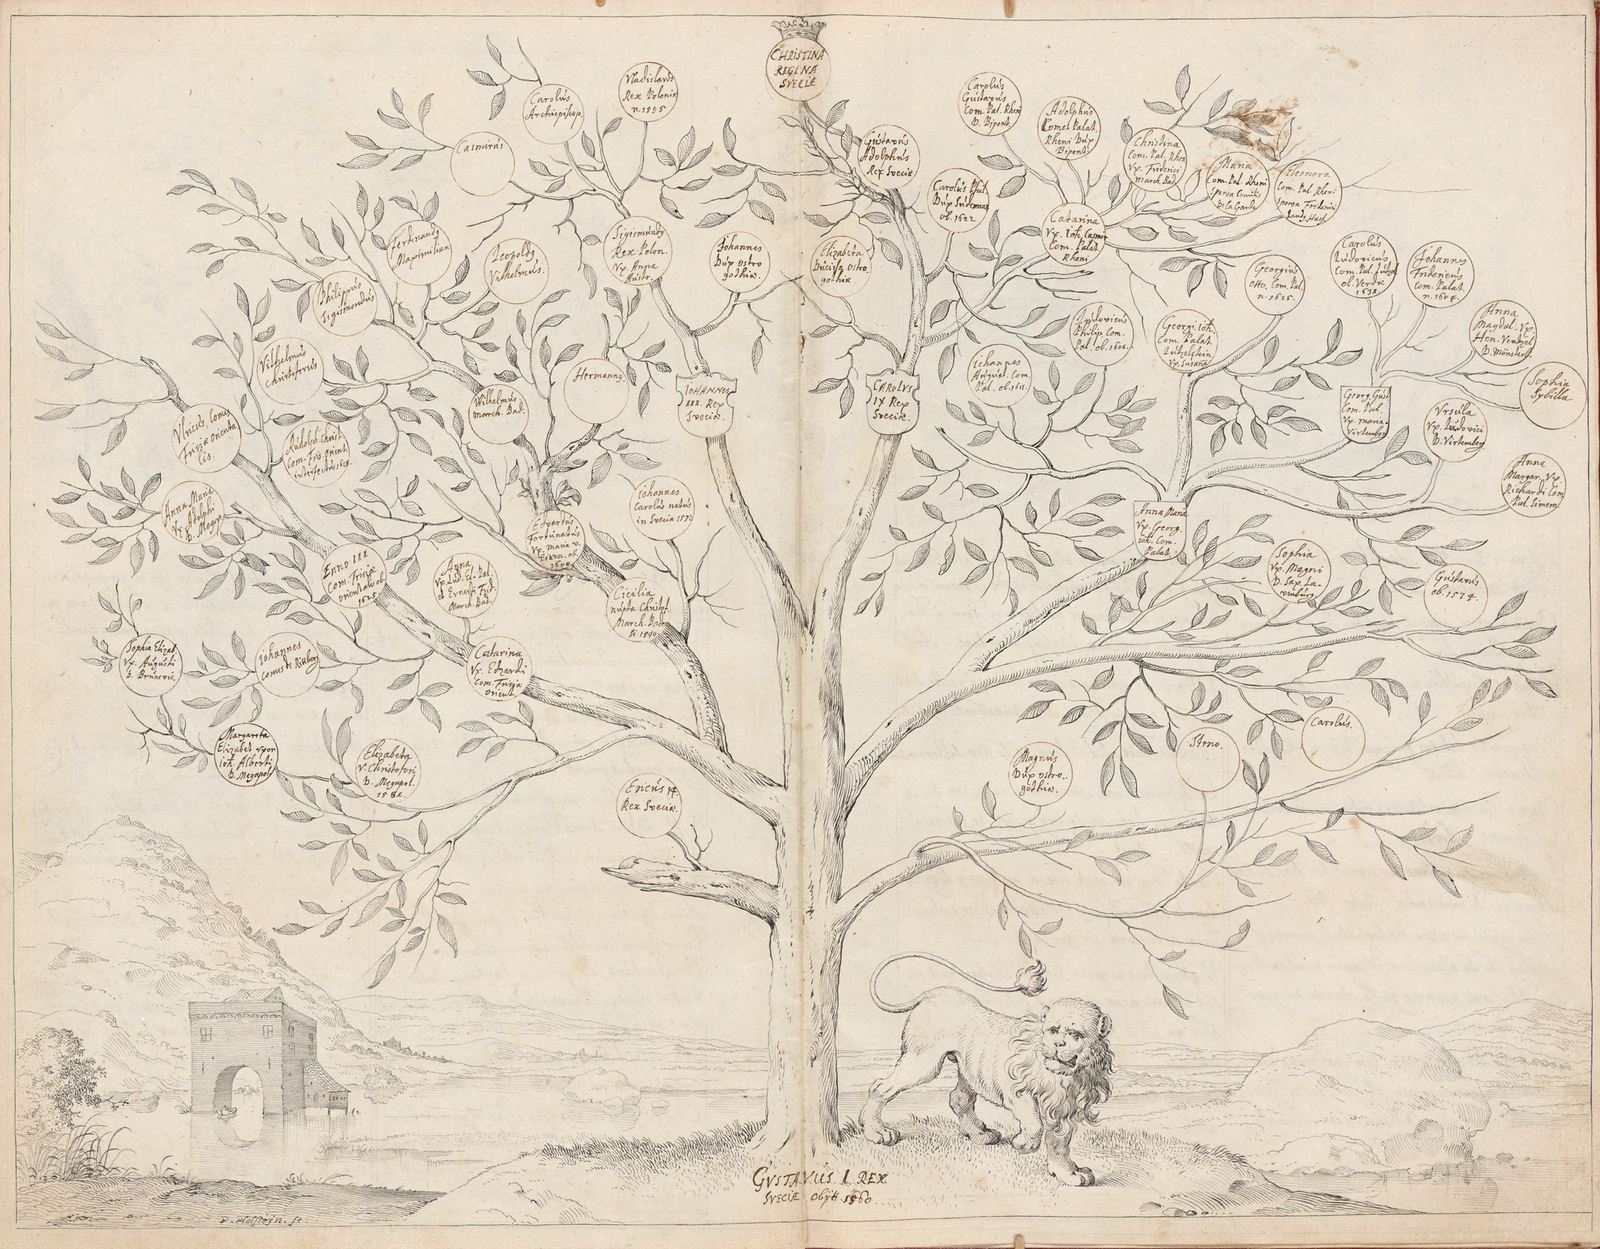
\includegraphics[width=\linewidth]{QueenChristinaLineage.png}
	\caption[Lineage of the house of Vasa from the \textit{Hortus Regius}]{Lineage of the house of Vasa from the \textit{Hortus Regius} or "Queen Christina's Genealogical Tree with Political Emblems".(\cite{hortusregius})} 
	\centering
	\label{queenlineage}
\end{figure}

When it comes to the subject of this work, the more relevant parts of the manuscript are the family trees. In \textit{Hortus Regius} there are nine genealogy charts depicting royal families in Europe at the time. The charts are drawn as trees with filigree leaves, and beautiful backgrounds and animals such as lions, horses and deer beside them. The ornaments probably holding meaningful symbolism.\footcite{hortusregius} Figure \ref{queenlineage} is a portrayal of the patrilineal tree of queen Christina and also the Vasa dynasty.

Gustavus Vasa "Gustavus I Rex" is found on the trunk of the tree. His children–including the female descendants–and their families are depicted as the branches. Gustavus Vasa's son and Christina's grandfather king Charles IX "Carolus IX Rex" and Christina's father Gustavus Adolphus "Gustavus Adolphus Rex" can be found near the treetop. Christina herself "Christina Regina" is on the top of the tree with a crown. 

Interestingly, some political picks are easy to spot on the genealogy chart of Vasa dynasty. The branch of Gustavus Vasa's son king Eric XIV (1533-1577) "Ericus 14 Rex(TODO check)" is broken violently leaving behind just a sharp cutting. In fact Eric was dethroned by his brother duke John (1537-1592, future king John III) and later poisoned.\footcite[pp. 118-124.]{MelinEtAl} Yet, no mention of Eric's two children with his wife of ignoble birth Karin Månsdotter can be found either. These political choises are understandable when thinking the family tree in its context. 

As a matter of fact, genealogy charts were of a high value to the aristocracy on the early modern timeperiod. Family trees were to prove the noble birth and blood, and therefore to legitimate the high status and rank (the position signed by God). The charts have been so valuable that in some cases they have been enhanced or even forged.\footcites[pp. 192-197]{friedrich18}[p. 150]{hakanenEtAll2020}[p. 158.]{lappalainen06} Family trees were politics. For example the long religious and civil wars forced the French noble families to reassess and redraw their affiliations with one another, and further with the monarchs in the latter half of the 16th century. While some European noble houses went so far, that they constructed a genealogy charts with biblical, Roman or Trojan heroes as their early ancestry, generally the practice of genealogy took a more critical and evidence-based stance towards the end of the 17th century.\footcite[pp. 192-197.]{friedrich18}

Ideally the aristocratic blood, possessions, position and wealth were inherited through patrilineal path, from father to son, but due the high child mortality in the early modern time, many families were left without legal inheritors. In fact many ennobled family lines died down during the 17th century.\footcite[pp. 158-160.]{lappalainen06} Possibly due the harsh realities of life's contingency and high child mortality, aristocrats in the early modern Sweden took the matrilineal heritage into account, and women were granted of inheritance of landed property.\footcites[p. 43]{lahtinen2020}[p. 40.]{lappalainen06} As an analogue, the \textit{Hortus Regius} has a delicate drawing of queen Christina's matrilineal heritages.\footcite{hortusregius}

Marriage was the another way of inheriting and uniting property and social status. According to Mirkka Lappalainen the noble marriages in the early modern period were mostly a mix of social opportunism with a genuine companionship and attraction between the spouses. The ideal of marriage was a harmonious companionship, and it was considered barbaric to force marriage, therefore forced marriages were of an exception. A rise in the social hirarchy through marriage was easier for women, and especially girls were tried to be married off to a suitor with a higher rank.\footcite[pp. 33-42.]{lappalainen06}

In the early modern Sweden divorce was not practically an option. Yet, because common illnesses like flu and states like pregnancy and childbirth could easily turn deadly, many marriages–happy or not–ended as Death did the couple apart. Usually aristocrats who lived till their 50s and 60s, had been married and wiodwed approximately two to three times during their lives. The marriages and remarriages formed large stepfamilies and larger family networks.\footcite[pp. 35-42.]{lappalainen06}

While marrying a cousin in the early modern Sweden was not illegal, it was considered weird and undesirable, the family networks were generally larger but more sparse. Instead of tightly knit network of one dynasty, the networks included plethora of notable families.\footcite[p. 40.]{lappalainen06} Mirkka Lappalainen approximates that in the 16th century the Swedish political elite consisted of around 20 families.\footcite[p. 55.]{lappalainen09} As marriages are an integral part of inheritance in the early modern Sweden the family links through marriage are not distinguished from the ones through blood in the Councillors of the Realm dataset or the graph depicting it.\footcite{councillorsDS}

Outside of marriage, but related through blood, the illegitimate children were an anomaly in the early modern society. Premarital and extramarital affairs were forbidden in the Swedish law and morale of the time. The law enforcement was however directed at the common people. Upper nobility was practically above of the law, and the scandals were taken care of discretely in private. While we do have evidence of a number of illegitimate children, many nobles were in fact deeply religious, and did not have affairs outside of the Holy Matrimony.\footcite[pp. 36-37.]{lappalainen06}

Illegitimate children are found in the Councillors dataset. For example Tore Jönsson Tre Rosor (id 231, died 1532) had his illegitimate son Jacob Turesson Rosengren (id 175, died 1571) in the council. Carl Carlsson Gyllenhielm (id 81, 1574-1650) was the illegitimate son of Charles IX, and Gustaf Gustafsson af Vasaborg (id 241, 1616-1653) was the illegitimate son of Gustav II Adolf.\footcite{councillorsDS}

As marriages, alliances and the art of genealogy were of a high value in the early modern culture, a compelling question is whether or not those family trees can be understood as networks. To get an intuitive opinion I have had unofficial discussions with my friends an colleagues about the subject matter and most of them have counted family trees as networks without doubt. Family trees also fit the mathematical criteria of a graph with nodes (persons) and directed edges (inheritance). Formally $G(V,E)$ where V means the vertices and E means the edges of graph G.\footcite[p. vii]{RajPM2018a}

Some text books have depicted family trees as an examples of simple networks.\footcite[See e. g.][p. 247.]{huhtamakiEtAl} While some scholars explicitly describes family trees as (sparse) graphs.\footcite{batagelj} Obviously, in early modern times family trees have not been used in the sense of network analysis or as analytical tools, as we know them today, but the contemporaries may have still been more familiar with the idea of network thinking than we may think.

\subsection{The Script}
For the conclusive analysis, I did some improvements to the Python script. The script is available in GitHub\footnote{\url{https://github.com/Heidi-Suurkaulio/mastersthesis/tree/main/PythonScript}} and can be found in Appendix \ref{script}. The viable version of the script is largely based on the test run script, however I added the functionality and did some refactoring; adjustments to make the code more slick. 

The scirpt reads and prints data in exactly same format as the previous one. The input data must be formatted similarily to the example of Table \ref{tab1} in the .csv format. However, the name of the input file is given as a command line parameter. The new functionality is that also the timerange of the network can be delimited with command line parameters. As a side-effect of the timerange functionality, the "ghost" nodes discussed in Chapter \ref{sources} are removed automatically.

The format of the command is as follows: 
\begin{verbatim}
python data_sifter.py Councillors_of_the_Realm1523-1680.csv
\end{verbatim}

This produces the network from the original time period given in the dataset. And, for example, command "\texttt{python data\_sifter.py <dataset.csv> prior 1650}" and "\texttt{python data\_sifter.py <dataset.csv> post 1590}" limits the networks to councillors and their relatives appointed before 1650 or after 1590. Lastly the command "\texttt{python data\_sifter.py <dataset.csv> 1540 1620}" delimits the network to councillors and their relatives appointed between 1540 and 1620.

When it comes to the script and the graph, I made some simplifications. The types of the relationships, such as brother, grandfather or brother-in-law, are not taken into account. Each relationship is taken from the dataset by the Id number and marked as an undirected edge with weight standard 1.0. This means that the graph does not separate blood relations, the relationships formed through marriages or illegitimate blood relations. As in the previous research, the family ties in general are mentioned to have been valuable, this graph depicts family ties as an abstraction.\footnote{See subsection \ref{background}.} 

The second simplification is that only the years of appointments are taken into account, but the years of death are not. Most of the time the position of the councillor was a lifelong.\footcite[TODO]{HakanenAKoskinen2017} So, the graph can not give a defined picture of the amount of the councillors active during a certain timeperiod. Basically the graph represents the family network of councillors appointed during certain timeperiod, and answers the question: \textit{Who were appointed to the Council and to which degree they were related to each other?} The script could be further develop into regognizing the type of the relationship and taking the years of death–the obvious end to the position–into account.

\subsubsection{Testing the Script}
Before anything else the script had to be tested. Testing is one of the most important–yet daunting–task in programming. Due the size and complexity of the Councillors dataset, the Python script is hard and ambiguous to test with the original data. To test the logic and behavior of the script I crated a small test dataset with simple dummy data. The test dataset is intentionally so small that it is readable by human. With the script the test dataset is available in GitHub.\footnote{\url{https://github.com/Heidi-Suurkaulio/mastersthesis/tree/main/PythonScript}} 

The test dataset consist of 12 entries with values for name, id number, (year of) appointment and family links. The names are represented by capital alphabets from A to L, and ids are sequential numbers from 1 to 12. The values in appointment-column are numbers between 1000 and 1299, and there are intentionally four entries within every range of 100. The family links are represented by numbers found in the ids except one which should be excluded by the script if everything works as planned. 

\begin{table}
	\caption{Example of the test dataset}
	\centering
	\begin{tabular}{cccc}	
		\hline
		Name; &Id; &Appointed; &Family\\
		\hline
		A; &1; &1000; &example 11\\
		\hline
		B; &2; &1000; &3, 4\\
		\hline
	\end{tabular}
\end{table}

When run with default setting the test dataset should produce 13 connections excluding the connection to the non-existent id 30, as it does. Giving the range 1000-1999, 1100-1199 and 1200-1299 as arguments divides the dataset in the groups of four as intended. Lastly giving the "prior 1150" and "post 1138" as arguments reduces the amount of entries and connections as expected. With the small test dataset the algorithm should work as intended. Inconveniently, the accuracy of the connections still has to be checked manually. 

The graph consisting of 257 nodes is way too complex for a human eyes and brain to inspect thoroughly. Therefore I compared parts of the connections in the largest graph with the connections in the dataset. This means that samples of the actual graph is checked by human. 

Lastly, to roughly review the results the script gives with the original dataset, I used some simple R script with R's ready-made functions to do some duplicate checking on the number of nodes. For the number prior to year 1600 the R script gave 111, and post year 1601 the R script gave 146. These are the R script gave the expected results.